% ======================================================================
% Module 5: real-data results (E5 held-out forecast, E7 rolling forecasts)
% Three frames, no title slide: \input this file into the main deck.
%
% Needs in the main preamble:  \usepackage{graphicx,booktabs,amssymb}
% Figures are in figs/ next to this file. If this file sits in a folder
% (e.g. module5/), add \graphicspath{{module5/}} to the main preamble.
% All numbers are from report/main.tex (final Colab run, WHO data).
% ======================================================================

% Method colours match the figures (pinn_figures.py, METHOD_STYLE)
\definecolor{mvPINN}{HTML}{7B2D8E}
\definecolor{mvPW}{HTML}{2A9D3A}
\definecolor{mvCB}{HTML}{1F5FBF}
\definecolor{mvInk}{HTML}{1F2933}
\definecolor{mvMuted}{HTML}{5F6B7A}
\definecolor{mvSoft}{HTML}{F3EDF6}
\definecolor{mvRule}{HTML}{C9B6D3}

\providecommand{\mvPINN}{\textcolor{mvPINN}{\textbf{PINN}}}
\providecommand{\mvPW}{\textcolor{mvPW}{\textbf{Piecewise-$\beta$}}}
\providecommand{\mvCB}{\textcolor{mvCB}{\textbf{Constant-$\beta$}}}
\providecommand{\mvTakeaway}[1]{%
  \par\vspace{3pt}\noindent
  \fcolorbox{mvRule}{mvSoft}{\parbox{\dimexpr\linewidth-2\fboxsep-2\fboxrule\relax}{\footnotesize\color{mvInk}#1}}}

% ----------------------------------------------------------------------
\begin{frame}{E5: Held-out forecast on WHO data}
\framesubtitle{Module 5 \textbullet\ WHO lab-confirmed reports, Sierra Leone \textbullet\ fit: 29 Aug 2014 -- 24 Feb 2015 \textbullet\ test: 25 Feb -- 25 Apr 2015, never seen}
\vspace{-2pt}
\begin{columns}[T,onlytextwidth]
\column{0.495\textwidth}
  \centering
  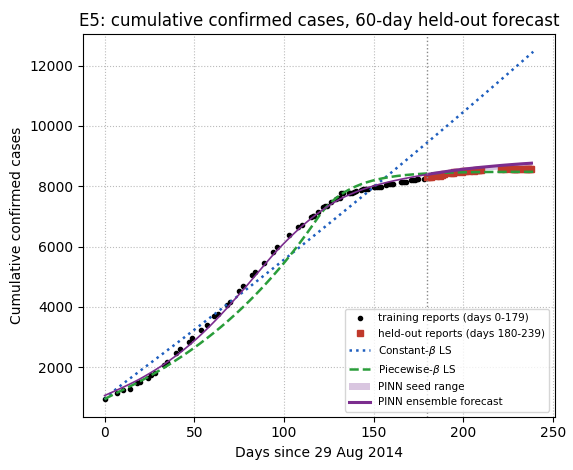
\includegraphics[height=0.54\textheight]{figs/e5_cases.png}\\[1pt]
  \scriptsize
  \begin{tabular}{@{}lccc@{}}
    \toprule
    Cases, relative error & \mvPINN & \mvPW & \mvCB \\
    \midrule
    60-day forecast & 1.35\% & \textbf{0.82\%} & 28.6\% \\
    \bottomrule
  \end{tabular}
\column{0.495\textwidth}
  \centering
  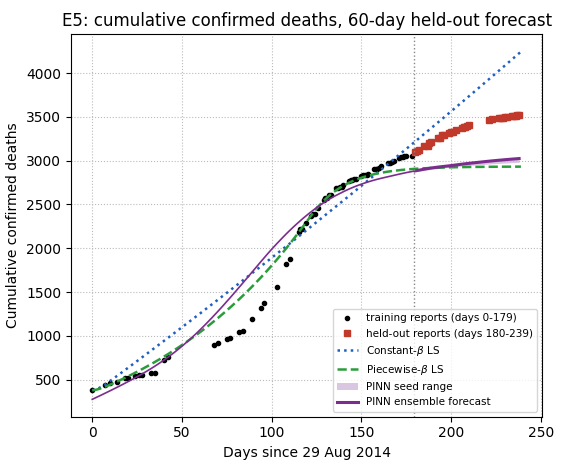
\includegraphics[height=0.54\textheight]{figs/e5_deaths.png}\\[1pt]
  \scriptsize
  \begin{tabular}{@{}lccc@{}}
    \toprule
    Deaths, relative error & \mvPINN & \mvPW & \mvCB \\
    \midrule
    60-day forecast & 11.8\% & 12.9\% & \textbf{10.7\%} \\
    \bottomrule
  \end{tabular}
\end{columns}
\mvTakeaway{\textbf{A time-varying $\beta$ is what matters:} \mvCB\ keeps growing and misses cases by 29\%.
\mvPINN\ is a close second to \mvPW\ on cases (single seeds: 0.28--1.75\%).
\textbf{Deaths defeat every method} (11--13\%): WHO added 463 deaths but only 361 cases in the test window.}
\end{frame}

% ----------------------------------------------------------------------
\begin{frame}{E7: Rolling 4-week forecasts across the epidemic}
\framesubtitle{Module 5 \textbullet\ 8 origins, every 28 days from 16 Jan to 31 Jul 2015 \textbullet\ each fit sees only the previous 8 weeks}
\vspace{-4pt}
\centering
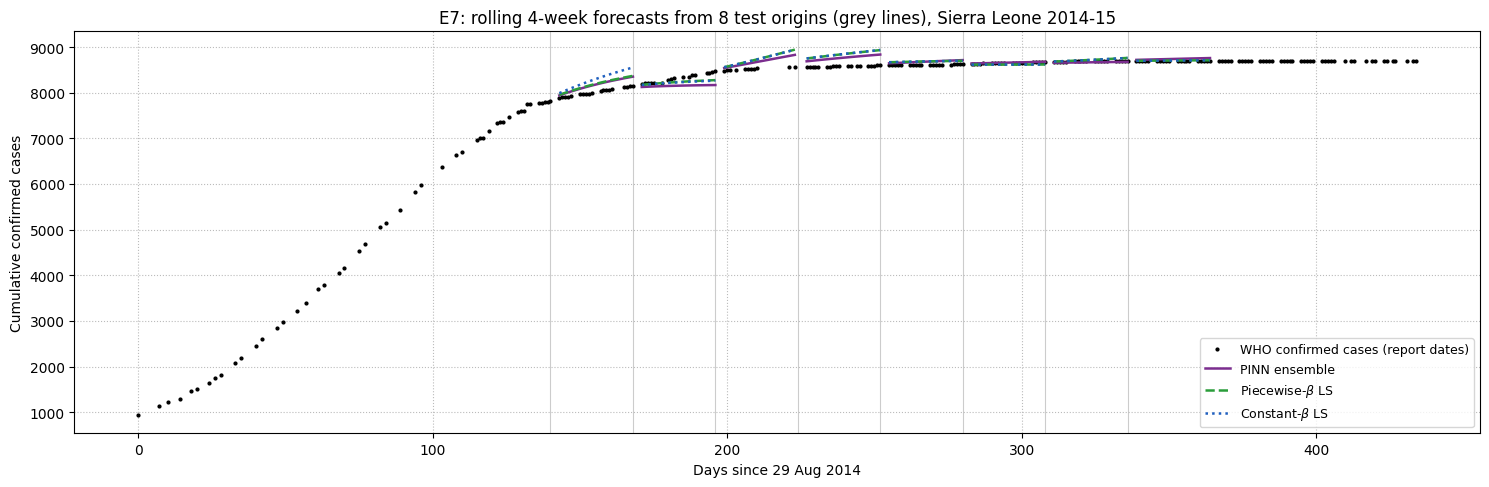
\includegraphics[height=0.52\textheight]{figs/e7_rolling.png}\\[3pt]
\begin{columns}[T,onlytextwidth]
\column{0.50\textwidth}
  \scriptsize\setlength{\tabcolsep}{4pt}
  \begin{tabular}{@{}lccc@{}}
    \toprule
    Mean of 8 origins & Cases MAE & New cases, 4 wk & Deaths MAE \\
    \midrule
    \mvPINN\ (3 seeds) & \textbf{96.8}  & \textbf{148.2} & 69.7 \\
    \mvPW              & 106.5          & 167.8          & \textbf{42.0} \\
    \mvCB              & 120.9          & 192.5          & 50.7 \\
    \bottomrule
  \end{tabular}\\[1pt]
  {\tiny\color{mvMuted} Errors in people. ``New cases, 4 wk'': error in new cases over the horizon.}
\column{0.46\textwidth}
  \footnotesize
  \begin{itemize}\setlength{\itemsep}{1pt}
    \item[$\checkmark$] \textbf{Cases:} \mvPINN\ is best on average, 20\% below \mvCB, and beats \mvPW\ at 6 of 8 origins.
    \item[$\times$] \textbf{Deaths:} \mvPINN\ is worst; its death forecast inherits any error in the learned $\mu$.
  \end{itemize}
\end{columns}
\end{frame}

% ----------------------------------------------------------------------
\begin{frame}{What the PINN adds, and what it costs}
\framesubtitle{Module 5 \textbullet\ interpretation and limitations}
\vspace{-2pt}
\begin{columns}[T,onlytextwidth]
\column{0.47\textwidth}
  \centering
  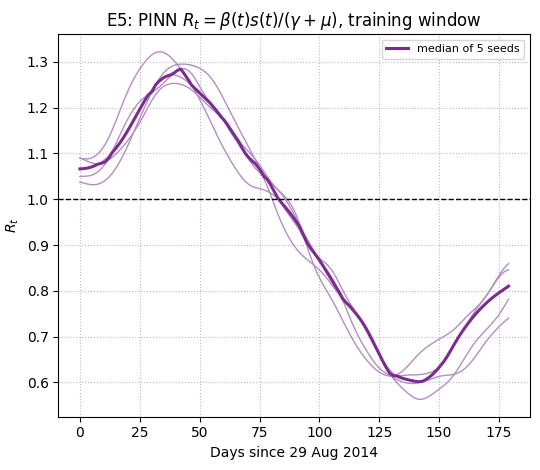
\includegraphics[height=0.49\textheight]{figs/e5_rt.png}\\[1pt]
  \scriptsize\raggedright
  \textbf{Learned $R_t = \beta(t)\,s(t)/(\gamma+\mu)$}, E5 training window (5 seeds, median bold):
  \begin{itemize}\setlength{\itemsep}{0pt}
    \item peak $\approx 1.28$ in early Oct 2014
    \item crosses 1 in mid-Nov 2014: the epidemic turns
    \item $\approx 0.6$ in mid-Jan 2015, $\approx 0.8$ by late Feb 2015
  \end{itemize}
\column{0.50\textwidth}
  \footnotesize\raggedright
  \textbf{\color{mvPINN}What it gives that least squares does not}
  \begin{itemize}\setlength{\itemsep}{1pt}
    \item a continuous $R_t(t)$ with no breakpoints to choose
    \item the case-fatality ratio, learned: 0.347--0.357 across seeds
    \item the hidden compartments $S, E, I$ alongside the fit
  \end{itemize}
  \vspace{2pt}
  \textbf{\color{mvMuted}What it costs}
  \begin{itemize}\setlength{\itemsep}{1pt}
    \item 1--2 min per fit (Colab CPU) vs.\ seconds for least squares
    \item needs a seed ensemble: single seeds vary (0.28--1.75\%)
    \item forecasts hold $\beta$ at its recent value, so they cannot foresee a new intervention or a resurgence
  \end{itemize}
\end{columns}
\mvTakeaway{\textbf{Honest verdict:} on cases the PINN forecasts about as well as the best classical fit; on deaths it does worse.
Its real value is an interpretable, continuous picture of transmission.}
\end{frame}
